\documentclass{article}
\usepackage{tikz}

\begin{document}

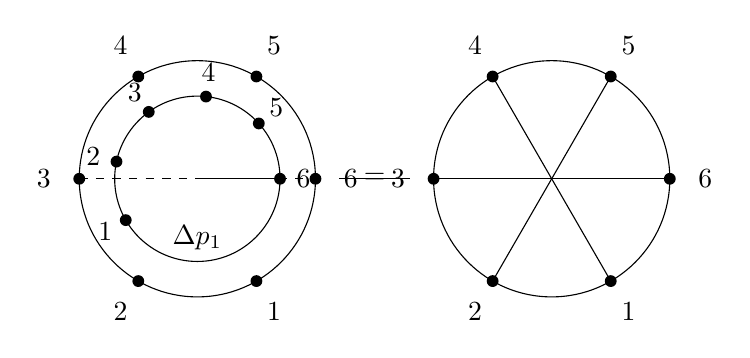
\begin{tikzpicture}[scale=1.5]
    % Draw the outer circle
    \draw (0,0) circle (1);
    
    % Label the points on the circle
    \foreach \angle/\label in {0/6, 60/5, 120/4, 180/3, 240/2, 300/1} {
        \fill (\angle:1) circle (0.05);
        \node at (\angle:1.3) {\label};
    }
    
    % Draw the inner circle
    \draw[dashed] (-1,0) -- (1,0);
    \draw (0,0) circle (0.7);
    
    % Label the points on the inner circle
    \foreach \angle/\label in {0/6, 60/5, 120/4, 180/3, 240/2, 300/1} {
        \fill (0.7*\angle:0.7) circle (0.05);
        \node at (0.7*\angle:0.9) {\label};
    }
    
    % Draw the line segment
    \draw (0,0) -- (0:0.7);
    
    % Add the label
    \node at (0,-0.5) {$\Delta p_{1}$};
    
    % Draw the equal sign
    \draw (1.2,0) -- (1.8,0);
    \node at (1.5,0) {$=$};
    
    % Draw the second diagram
    \begin{scope}[xshift=3cm]
        % Draw the outer circle
        \draw (0,0) circle (1);
        
        % Label the points on the circle
        \foreach \angle/\label in {0/6, 60/5, 120/4, 180/3, 240/2, 300/1} {
            \fill (\angle:1) circle (0.05);
            \node at (\angle:1.3) {\label};
        }
        
        % Draw the lines from the center to the points
        \foreach \angle/\label in {0/6, 60/5, 120/4, 180/3, 240/2, 300/1} {
            \draw (0,0) -- (\angle:1);
        }
    \end{scope}
\end{tikzpicture}

\end{document}